\documentclass[twocolumn,a4paper]{IEEEtran}
\usepackage{graphicx}
\usepackage{ amssymb }
\DeclareGraphicsExtensions{.eps,.ps,.jpg,.bmp}
\pagestyle{headings}
\title{Planning of virtual power plant considering dispatchable load under uncertainty}
\author{Changyu Zhou}

\begin{document}
\maketitle
\begin{abstract}
Virtual power plants (VPP) are expected to be important components of the new intelligent energy. 
In this study, a two-stage stochastic optimization model is developed for the planning electric power systems included VPP under uncertainty. 
The support vector regression technique is applied to the prediction of power demand. 
The prediction result is then used in the planning model peak load constraints. 
The model systematically reflects the complexity of the renewable energy management system and improves the applicability of the modeling process. 
The resulting solution provides the desired energy resource/service allocation plan with minimized system costs, maximized system reliability, and maximized energy security. 
And thus the trade-off between system costs and energy security will balance. The results show that the dispatchable load of the virtual power station can effectively alleviate the power generation pressure caused by the shortage of renewable energy due to weather and other factors. 
In detail, this study aims to provide: 
(a) adjustment or justification of the pattern of distribution of renewable energy resources and services in the context of Intelligent Energy; 
(b) decision support of local policies on energy use, economic development and energy structures under various energy supply and policy interventions; 
(c) analysis of the interaction between economic costs, system reliability and energy supply shortages. 
\end{abstract}
\begin{IEEEkeywords}
Virtual power plant, Uncertainty, Electric power systems, Interval, Support vector regression
\end{IEEEkeywords}
\section{Introduction}

China is the world's largest consumer of energy and electricity. 
The overall power supply is abundant in China. 
Nevertheless, due to uneven development, the electricity shortage still exists in some areas during the peak period of electricity consumption [1], 
whereas some capacity is idle at the low-load period in these areas. 
This phenomenon not only increases the power costs and pollution emissions in the peak-period but also caused the resource waste in the low-load period. 
On the other hand, China's government is actively adjusting the structure of energy, 
optimizing the power production structure and further improving the proportion of non-fossil energy generation. 
The installed power generation capacities of hydro, wind and solar in China rank the first around the world [2]. 
The intermittent and unpredictable nature of clean energy generation, 
such as wind power and photovoltaic power generation, increases the cost and risk of renewable energy grid-connected. 
How to improve the stability of renewable energy grid-connected? 
How to deal with the problems of energy shortage, environmental pollution? 
How to adjust the user's power consumption, reduce the peak and valley difference, and ensure the safe and stable supply of electricity for the power system? Solve those urgent problems are vital for China and the world to move forward with a clean, efficient, safe and sustainable energy development. 
Under the above background, VPP is proposed as a new technology for smart energy in the power market. 
VPP refers to heterogeneous power plants, which usually include heterogeneous distributed energy resources (DERs), traditional fossil fuel power plants, energy storage facilities and dispatchable loads, as shown in Figure 1. 
According to the characteristic of the service region, its concrete composing form is various. 
The VPP can effectively integrate, aggregate and manage traditional and renewable energy power plants, including distributed generators, energy storage systems and dispachable loads [3], in order to increase the power generating, reduce the instability of wind and solar power generation, shave peak load to cope with power shortage during rush hour. 

\begin{figure}
    \centering
    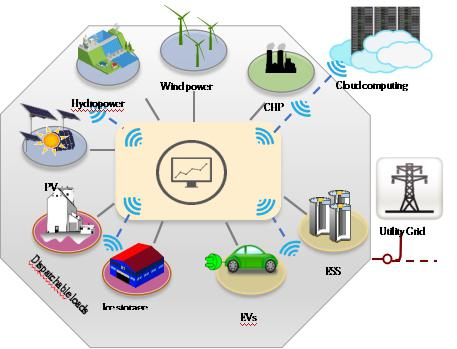
\includegraphics[width=0.5\textwidth]{figure/figure1.jpg}
    \caption{The composition of heterogeneous VPP}
    \label{The composition of heterogeneous VPP}
\end{figure}


In Europe, there are many demonstration projects of VPP, shown in table 1. 
For instance, the Danish EDISON VPP(EVPP) project [4] collects historical data and real-time data on the operation of electric vehicles, and aggregates them to form the market resources, then participates in the market transaction through the retailers. 
The European Union's FENIX-VPP project [5] is a combination of traditional generator sets and cogeneration of wind turbine generator to form VPP, coordinated and controlled through technical means, and then involved in the electricity market through trading software. 
The EU's WEB2-ENERGY-VPP project [6] attempted the transmission of the electricity communication protocol IEC61850 in a wide area network. 
End users and power supplies can be accessed via the Internet into the control center of the VPP, and through the CIM-61850 converter is converted into an electric public information model to participate in market transactions. 
The Netherlands Power Matcher(PM) [7] architecture is a kind of agent concept, that is, the VPP can assume a centralized agent, auction agent, and other different agent functions, in the market to gain profits. 
In Germany, there are several VPP projects such as the vpp-intelligent-energy, etelligence, and RegModHarz[8]. 
The smart grid pilot project eTelligence, which combines large ice storage as a dispatchable load and wind power plants to form a VPP. 
By adopting the policy of combination of segmented electricity price and dynamic electricity price, the load of the two ice storages will be adjusted automatically with the power fluctuation of electricity price and wind power. 
The standard of OPENIEC61850 communication protocol based on etelligence project design has been recognized by the German industry. 
The PREMIO project is used to optimize the effect of module access such as distributed energy, storage and demand response in power grids [9]. 
The "large-scale and friendly interactive system" in Suzhou, China, can carry out millisecond control on several interruptible loads, and by cutting off some unimportant small power supply, the priority to ensure the important load will not be affected when the instantaneous power outage of the power grid. 

\begin{table}
\tiny
\setlength{\tabcolsep}{3pt}
\begin{tabular}{|c|c|c|c|c|c|c|c|c|c|}
\hline
Project&\multicolumn{8}{|c|}{VPP Members}&Function\\\cline{2-9}
&PV&WPP&PSH&CPP&CHP&ESS&EV&DL&\\
\hline
EDISION&&\checkmark&&&\checkmark&&\checkmark&&PBDR+FR\\
\hline
PowerMatcher&&&&&\checkmark&&&&PS\\
\hline
FENIX&\checkmark&\checkmark&&\checkmark&\checkmark&&&\checkmark&PBDR+PS+FR\\
\hline
WEB2ENERGY&\checkmark&\checkmark&\checkmark&&\checkmark&&&\checkmark&PBDR+IRC+FR\\
\hline
eTelligence&\checkmark&\checkmark&&&\checkmark&&&\checkmark&PBDR+IBDR+PSFR\\
\hline
vpp-intelligent-energy&\checkmark&\checkmark&&&\checkmark&&&\checkmark&FR\\
\hline
RegModHarz&\checkmark&\checkmark&\checkmark&&\checkmark&&\checkmark&&PBDR+PS\\
\hline
PREMIO&\checkmark&&&&&\checkmark&&\checkmark&PS\\
\hline
\end{tabular}
\caption{The structure and function of demonstration projects of VPP}
\end{table}


In addition to the above-mentioned practical demonstration projects, scholars have carried out a lot of research work on the technical feasibility, economic feasibility, and reliability of the VPP. 
In [10], the authors put forward a technique of dispatching and optimizing operation, integrating the data center into Intelligent Power network to participate in the intelligent demand response, and the simulation results verify the feasibility of the technology. 
A distributed VPP scheduling method without centralized control center is proposed in [11]. 
The authors in [12] analyze selected communication quality of service parameters, in particular, latency, packet loss, retransmissions, bandwidth, amount of traffic, and message patterns of the IEC 60870-5-104 protocol. 
Authors of [13] proposed a VPP routing algorithm for data communication, which supports centralized, decentralized, or fully distributed control. 
These studies provide technical support for the participation of VPP in the flexible response of power market transactions. 
LI et al. [14] discussed the feasibility and incentive mechanism of a VPP based on the case of Chongming in China. 
The results show that the optimal combination ratio of wind energy and photovoltaic power stations is conducive to raising the self-sufficiency rate of Chongming Electric Power. 
In [15] the authors conclude that explores the development of Germany's future energy system, and the simulation results show that the heterogeneous VPP composed of fossil power plant, renewable energy, and cogeneration equipment can bring some economic benefits. 
Based on the bid information of Korea Electric Exchange, authors of [16] puts forward a demand response method of the VPP, and tests and validates the method in IEEE Reliability Test System (IEEE RTS-24). 
The results show that the method can bring down the total operating cost. A method of VPP scheduling management optimization model for maximizing the profit is presented in [17]. 
The operator can select the best demand response loads program for each VPP in a scheduling procedure, and the reliability of the model is also tested in IEEE RTS. 
In [18] takes the VPP as the production/the consumer to participate in the market transaction independently, also takes the VPP profit maximization as the goal, proposed the two-stage stochastic mixed integer linear programming model under electric power market planning. 
In [19-21] establishes the optimal dispatching model in the power market environment in which traditional power plants, renewable energy power plants and VPP coexist. The problem of the cooperation between neighboring VPP is discussed in [22], to maximize the expansion of VPP's energy trade opportunities. 
Authors of [23] take Genco as an example to establish the optimal operation scheme of risk avoidance in the VPP is established. These studies further confirm the feasibility of the VPP participating in energy trading and distribution issues. 
In addition, there are a few studies on the involvement of smaller energy efficiency units in the power market. In [24] author constructs a virtual energy storage system that stores and releases energy by coordinating the demand response of the city's household refrigerators to achieve the goal of reducing carbon emissions by replacing the rotational reserve capacity of fossil-fueled generators. 
The study of the VPP or energy-efficient power plant provides a new direction for solving the problem of power supply shortage, energy supply security and energy integration. 
In particular, the rapid development of smart grid technology promotes reasonable resource configuration and provides solid support for VPP operation.

At present, the research on the VPP focuses on the operational frame, optimal dispatch, technology realization and operation control. 
However, many economic, environmental and policy factors have had a significant impact on the energy management process, leading to various uncertainties in decision-making. 
Dozens of system parameters (such as renewable resource availability, facility capacity, production efficiency and allocation target, as well as their interrelationships) may appear uncertain and may be presented in fuzzy, probabilistic and/or interval formats. 
Previous research on VPP rarely considered these uncertainties. 
Also, for VPP that contain controlled loads, decision-makers may need to know the following issues. 
What impact does a VPP with a controlled load have on a region's CO2 emissions? 
What kinds of power generation technologies are needed to meet these needs if the electric demands during peak periods are not shaved? 
In 2015, the growth rate of thermal power in China dropped by 2.6%, but in 2016, it increased by 3.6%. 
Can the peak load regulation by the VPP reduce the electric generating of fossil fuel power plants? 
What is the effect of load shifting? 
There are few reports about the mid-term effects brought by the VPP. 
Decision-makers need to comprehensively assess the combined impact of a VPP when formulating regional development plans.

Therefore, in this study, we will discuss the energy planning problem considering large ice storages as dispatchable loads incorporated with renewable energy power plants to form VPP. 
A power planning model based on the cost minimization strategy is proposed. 
The economic and emission reduction benefits of the energy substitution scheme, which is provided by using the intelligent incentive control mechanism in the smart grid, are analyzed.


\section{Modeling formulation}
This study will discuss the energy planning of VPP composed of dispatchable loads (such as large ice storage) and wind power generation, photovoltaic power generation and hydropower. 
Large-scale ice storages, freezers in supermarkets, or refrigerators and freezers in private homes can be viewed as electrical power facilities that store electricity in cold form. 
Hot-Spring convalescent facilities using cogeneration systems store electricity in hot form, and electric cars in cities can also be used as energy storage devices in the Smart Grid. 
These facilities all have sponge-like properties, they can play a role of energy storage when the power load is at a low point (i.e., the generating capacity is higher than the load), absorb and store electricity, and when the load is at a peak period (i.e., the generating capacity is less than the load), it is like energy storage device that begins to release electricity. 
Such as ice storage even if the power cut-off, the temperature drop is very slow, in a certain temperature and time range, and will not lead to the deterioration of the quality of storage goods. 
Therefore, can be opened according to load demand, low-load operation or shutdown. When the wind power is strong, solar energy is abundant and electricity market price is low, the smart control system can start the ice storage or reduce the set temperature of refrigerated in operation, to store a certain amount of electricity in 'cold' form. 
In the period of electricity shortage, lack of wind or solar energy and high price in the electricity market, smart system can suspend the operation of ice storage, run the frequency converter or increase the set temperature, to reduce the power consumption and play the role of peak load shifting. 
The traditional energy-efficient power plant and energy efficiency demonstration project are through the implementation of a package of the energy-saving plan, access to demand-side savings of power resources. 
A VPP with dispatchable load type is different, these "virtual power units" with their spongy properties do not reduce their demand for electricity or even increase the demand for electricity due to frequent start-up and shutdown of equipment. 
It only reduces peak electricity demand in the form of load transfer. 
In the power gap period, the "VPP" in some special areas can play an active role in regulating, such as areas where high reliance on renewable energy sources, port cities with many large-scale ice storages bases, and hot spring convalescent facilities using CHP systems.
The framework of VPP participating in energy market transaction is put forward, as shown in Fig.2. 
The large-scale ice storage in the VPP can serve as the peak shaving function.

As volatility and uncertainty increase dramatically because of more renewable energy grid-connected. 
In the power system planning, many data obtained will be biased, and the probability distribution and membership function of these data are not easy to obtain. 
ILP is an effective method to deal with uncertainties existing as interval values without distribution information [25,35-37]. 

There is an uncertain deviation between the actual output and the planned output of the power system dispatching wind power, PV, and hydropower with renewable energy. 
If the failure to achieve the planned output due to weather or other factors occurs, there will be a deviation penalty cost. 
At the same time, the power system also needs to arrange standby fossil fuel generating unit to generate electricity to meet the demand. 
The large ice storage, commercial buildings and other interruptible loads can be used as a part of the reduction of the output deviation of the renewable generations. 
Also, it can combinate with the renewable energy generation to form a VPP. 
The start-up and stopping of large ice storages will result in some economic losses. 
Thus, it is necessary to include the compensation cost of the deviation penalty cost and interruptible load into the objective function.

\begin{equation}
minf^\pm = min(f_1^\pm+f_2^\pm+f_3^\pm+f_4^\pm)
\end{equation}

\begin{equation}
f_1^\pm=\sum_{t=1}^3\sum_{k=1}^2CER_{t,k}^\pm \times AER_{t,k}^\pm
\end{equation}

\begin{equation}
f_2^\pm=\sum_{t=1}^3\sum_{i=1}^2\sum_{s=1}^4\sum_{d=1}^4 AEG_{t,i,s,d}^\pm \times CVG_{t,i}^\pm +\sum_{t=1}^3\sum_{i=1}^2 CFM_{t,i}^\pm \times ICA_{t,i}^\pm
\end{equation}

\begin{equation}
f_3^\pm=
\end{equation}


The annual power demand forecast is an important part of power system planning, which is influenced by economic and social uncertainties. Also, annual historical data is less. Support-Vector-Machine(SVM) is a machine learning method based on the principle of structural risk minimization. The basic idea is to transform the input space into a high-dimensional space by using the nonlinear transform defined by the inner product function and to find the exact description of the non-linear relation between the input variables and the output variables in this high-dimensional space. Support-Vector-Regression(SVR)can be applied to the prediction problem in the case of finite samples. Thus, SVR can be used for predicting electricity demand.

\end{document}